\scanpage{134}

1\deleted{2}\handwritten{3}) Useful variant of the carpet of number 6. Let $C$ be a category, and $\deleted{\unsure{F:C\;\mathrm{Mo}|F:C\;\mathrm{Mod}}}$
\[
F:C\handwritten{\longrightarrow}\mathrm{Modf}(k)
\]
a functor, where $\rlap{\(j\)}k$ is a field. We do not assume $C$ additive, nor $F$ faithful. We then define the profinite ring $U=\mathrm{End}_{k}(F)$, the dual coalgebra $A$, and we find a canonical factorization of $F$ through $\mathrm{Modf}(U/k)=\mathrm{Comodf}(A/k)$. Suppose given in $C$ a bifunctor $\unsure{\otimes|\Omega}$, \deleted{t\unsure{\rlap{t}h|h}en}\inserted{\handwritten{and}} an isomorphism of bifunctors $F(X\otimes Y)\handwritten{\simeq}F(X)\otimes F(Y)$, then we find a diagonal map on $U$ i.e. a composition law \deleted{\unsure{compatible|compatible} with \unsure{map}} on $A$: indeed, we observe that the endomorphism ring of the bifunctor on the left-hand side is $U\otimes_{k}U$, and $U$ map\rlap{e}s into it thanks to the given isomorphism $F(X\otimes Y)\handwritten{\simeq}F(X)\otimes F(Y)$. If for $\otimes$ we specify unit, associativity or commutativity data, the compatibility of these data with $c$ is then expressed as stated in number 6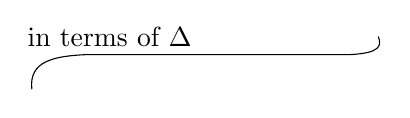
\begin{tikzpicture}[baseline=-.6ex,x=1cm,y=1cm]
\node[anchor=west,inner sep=0] at (0,.42) {\inserted{\handwritten{in terms of $\Delta$}}};
\draw (.06,-.24) .. controls (.02,.12) and (.34,.18) .. (.75,.2) -- (4.1,.2) .. controls (4.5,.22) and (4.5,.32) .. (4.46,.43);
\end{tikzpicture}, and one should give graded variants (if possible more general\handwritten{s} and clever\handwritten{s} than in number 8\handwritten{!)}. In fact, the results specific to number 6 would be \unsure{ra\rlap{t}ther|rather}, in the case of a fa\rlap{d}i\rlap{d}thful functor (and additive \deleted{of categories} exact of abelian categories ? to see exactly what is needed), converses to the preceding constructions, i.e. how to deduce from a diagonal map on $U$ a\deleted{e} functor $\otimes$ on $C$, wh\rlap{j}ose pr\rlap{i}operties will reflect those of the latter.

Interesting example: cohomology operations on $\underline{F}_{p}$. It deserves some explanations: except for the piece generated by the $\handwritten{\pi}_{i}$ \deleted{(NB $i$} the degrees in $U$ are $\handwritten{>}$ $0$, and $\overset{\handwritten{\sim}}{U}\text{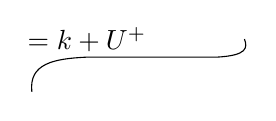
\begin{tikzpicture}[baseline=-.6ex,x=1cm,y=1cm]
\node[anchor=west,inner sep=0] at (0,.42) {\inserted{\handwritten{$=k+U^{+}$}}};
\draw (.06,-.24) .. controls (.02,.12) and (.34,.18) .. (.75,.2) -- (2.4,.2) .. controls (2.8,.22) and (2.8,.32) .. (2.76,.43);
\end{tikzpicture}}$ is the c\unsure{\rlap{n}a\rlap{n}a|aa|an|na}onical completion of a graded ring with an anticommutative diagonal map, so $\overset{\handwritten{\sim}}{A}$ is an analogous ring. Say how to recover $U,A$ from $\overset{\handwritten{\sim}}{U}$, $\overset{\handwritten{\unsure{\sim}}}{\overset{\handwritten{\sim}}{A}}$.
% archive sheet number: 133
